\section{Tablebases}
\label{sec:Tablebases}

\subsection{Overview}
As of writing this paper the largest available and widespread Tablebase is the Syzygy 7 man Tablebase \cite{syzygy}, it contains evaluations for all possible positions that could arise from having up to 7 pieces on the board (7 pieces in total including the kings). To download such a Tablebase, one would need to allocate somewhere around 16TBs of storage space, and if this is not possible, one could also generate these tablebases locally. For that one would \textit{only} need a machine with 1TB of RAM and it would take many decades of computing time.

Although they provide a very accurate evaluation for every one of those positions, the monstrosity of these tablebases makes their use obsolete for the average person. This is of significance, because anyone could download Stockfish \cite{stockfish2024}, one of the strongest chess engines of today, and have it immediately available on their machine for use at anytime. Although tablebases aid chess engines like stockfish in directing a position towards a favourable endgame, the high storage demands of tablebases raises the question, whether it would be possible to specifically create an engine that specialises in endgames, and alongside that remove all need for tablebases.

\subsection{The make up of a Tablebase}
Tablebases are large databases containing all possible (and legal) chess positions that could arise from having a certain amount of pieces on the board. For each of those positions, retrograde analysis \cite{retroAnalysis} is used to determine whether the outcome is a win, draw or loss.

Retrograde analysis works by taking a terminated position where one side is mated, and going backwards to discover all the possible positions that eventually lead up to the root position. This process is repeated for all mate positions for a given number of pieces, and subsequently a subdatabase of all possible positions that terminate in a mate are generated. Any other position that is still legal and valid but not found in the subdatabase is then marked as a draw.

\begin{figure}[H]
    \centering
    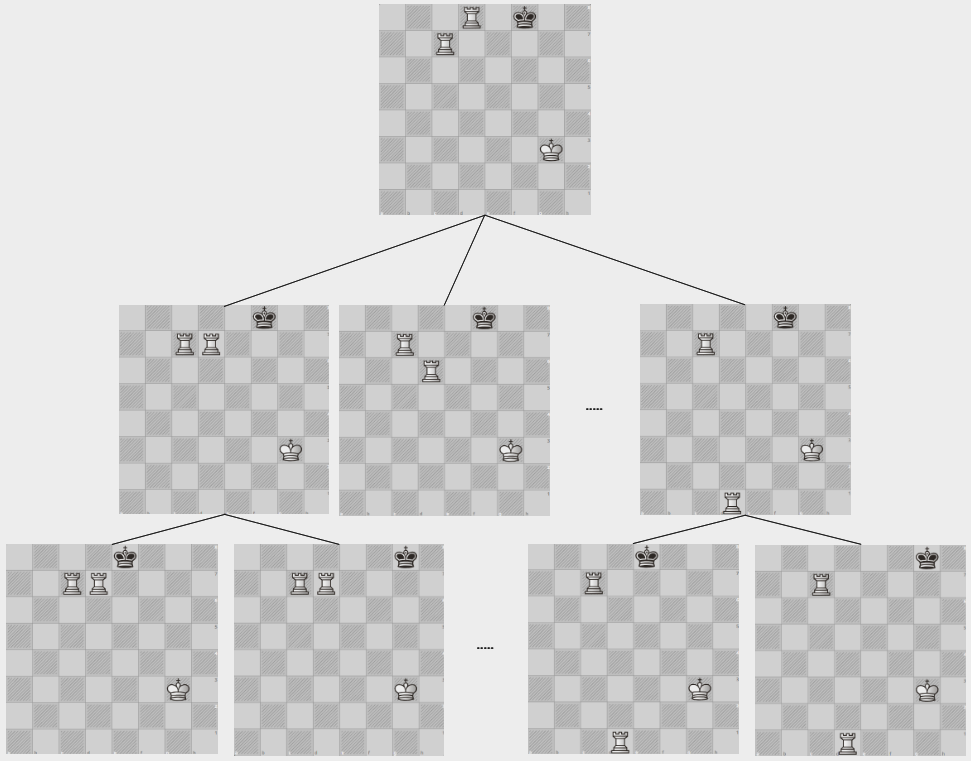
\includegraphics[scale=0.45]{images/retrogradeAnalysis.png}
    \caption{Simple visualisation of Retrograde Analysis}
    \label{rtroAnalysis}
\end{figure}

\subsubsection{Metrics}
Whether a move leads to a checkmate or not is ultimately the main measure of how good a move is, but there are several other aspects one could consider on the way to a move that leads to checkmate. For instance, when no mate can be found, a move that leads to resetting the 50 Move Counter \cite{50Draw} could point in the direction of eventually finding a mating move.



Few of the metrics that are commonly stored within tablebases are explained below:

\begin{itemize}
    \item \textbf{WDL}: The \textbf{W}in \textbf{D}raw \textbf{L}oss metric returns an integer number describing the evaluation of a given position. The possible values that can be returned are:
        \begin{itemize}
            \item \textbf{2}: The given position is won.
            \item \textbf{1}: The given position is drawn due to the win being prevented by the 50 move rule. This is also known as a cursed win.
            \item \textbf{0}: The given position is drawn.
            \item \textbf{-1}: The given position is drawn due to the loss being prevented by the 50 move rule. This is also known as blessed loss.
            \item \textbf{-2}: The given position is lost.
        \end{itemize}
    \item \textbf{DTM}: The \textbf{D}epth \textbf{T}o \textbf{M}ate metric returns an integer number indicating how many moves the winning side has to make in order to reach mate.
    \item \textbf{DTZ}: The \textbf{D}epth \textbf{T}o \textbf{Z}eroing metric works similarly to DTM but with the objective of reaching a capture or a pawn move, why these are important is made clear with the next metric.
    \item \textbf{DTZ50}: The \textbf{D}epth \textbf{T}o \textbf{Z}eroing in the context of the \textbf{50} move rule metric is an extension of the DTZ metric with keeping in mind that the capture or the pawn move must occur within 50 moves so that a draw is avoided.
\end{itemize}

Depending on the simplicity of the program being developed and the performance sought after, one need not use all the metrics available, and it would suffice to only use one. This is of importance due to the large accumulative size of the files for each metric. In the case of the 6-man Syzygy Tablebases used in the development of the programs accompanying this paper \cite{NeuralBases}, the WDL files alone measure to around 70GBs and they are sufficient to providing a solid base of probing the tablebase to aid in finding the best move in a position. This would save around 80GBs of additional storage space that would've been needed for the DTZ files.

\subsection{Probing}
Each position is assigned to an index that points to where the metrics such as WDL, DTZ, and others are stored for that specific position. In order to retrieve this information one would need to \textit{probe} the tablebase files.

Probing consists of applying the chosen indexing algorithm of a tablebase on the given position. Once the unique index is calculated, it is used to locate where the metrics of that position are stored in order to extract them \cite{chesswikiEGTB}.

Since the objective of this paper focuses on alternatives for tablebases the implementation of this part, was left out and the publicly available library Python-Chess \cite{pychess} was used in dealing with the Syzygy 6-man WDL Tablebases.. This library was chosen due to its developer being involved with most of the Syzygy Tablebases related aspects of the chess website Lichess and created the web API for using Syzygy Tablebases \cite{lichess}\cite{syzygyAPI}.